\chapter{Regulator DMC}
\label{zad4}


\section{Algorytm działania}
Algorytm działania regulatora oraz implementacja została dobrze udokumentowana w pliku \verb+DMC_Z.m +. Listing jego częsci algorytmicznej przedstawiony jest poniżej:
\begin{lstlisting}[style=custommatlab,frame=single,label={zad4_sim_lst},caption={Implementacja regulatora DMC},captionpos=b]

function [Err] = DMC_Z (paras)
% zmienne i macierze regulatora
load('odp_skok');
D=paras(1);
N = paras(2);
Nu=paras(3);
lambda = paras(4);
DZ = 25;
s = su;
z = zeros(N,1);
z(1:size(sz))=sz;
z(size(sz):end)=sz(end);

M=zeros(N,Nu);
for i=1:N
for j=1:Nu
if (i>=j)
M(i,j)=s(i-j+1);
end
end
end

MP=zeros(N,D-1);
for i=1:N
for j=1:D-1
if i+j<=D
MP(i,j)=s(i+j)-s(j);
else
MP(i,j)=s(D)-s(j);
end    
end
end

MZP=zeros(N,DZ);
for i=1:N
MZP(i,1) = z(i);
for j=2:DZ
if i+j-1<=DZ
MZP(i,j)=z(i+j-1)-z(j);
else
MZP(i,j)=z(DZ)-z(j);
end      
end
end

I=eye(Nu);
K=((M'*M+lambda*I)^-1)*M';
ku=K(1,:)*MP;
kz=K(1,:)*MZP;
ke=sum(K(1,:));
deltaup=zeros(1,D-1);
deltazp=zeros(1,DZ-1);

% dane
n = 200;
U0 = 0;
Z0 = 0;
Y0 = 0;
start = 10;

U = U0*ones(1,n);
Z = Z0*ones(1,n);
Z(100:end) = 1;
Y = Y0*ones(1,n);
Yz = Y;
Yz(10:end) = 1;
e = zeros(1,n);

%hold on
for k = start:n
Y(k) = symulacja_obiektu4y(U(k-6),U(k-7),Z(k-2),Z(k-3),Y(k-1),Y(k-2));
e(k) = Yz(k) - Y(k);

%uwzglednianie zaklocenia
for i = DZ:-1:2
deltazp(i) = deltazp(i-1);
end
deltazp(1) = Z(k) - Z(k-1);

% Prawo regulacji
deltauk = ke*e(k)-ku*deltaup'-kz*deltazp';

for i = D-1:-1:2
deltaup(i) = deltaup(i-1);
end
deltaup(1) = deltauk;
U(k) = U(k-1)+deltaup(1);
end
Err = (Yz-Y)*(Yz-Y)';
end

\end{lstlisting}


\section{Strojenie regulatora DMC}


Strojenie regulatora przeprowadzone zostało metodą automatyczną przy użyciu\\ funkcji \verb+ga(@DMC,nvars,[],[],[],[],lb,ub,[],IntCon,options)+. Strojonymi parametrami były $N$, $N_u$ oraz $\lambda$. Za dolne ograniczenie przyjęte zostały wartości $N=1$, $N_u = 1$, $\lambda = 1$, natomiast za górne $N=D$, $N_u = D$ oraz $\lambda = 1000$, gdzie $D = 116$. Wyniki strojenia regulatora przedstiowone są na wykresie \ref{fig:strojenie}.

\begin{figure}[h!]
	\centering
	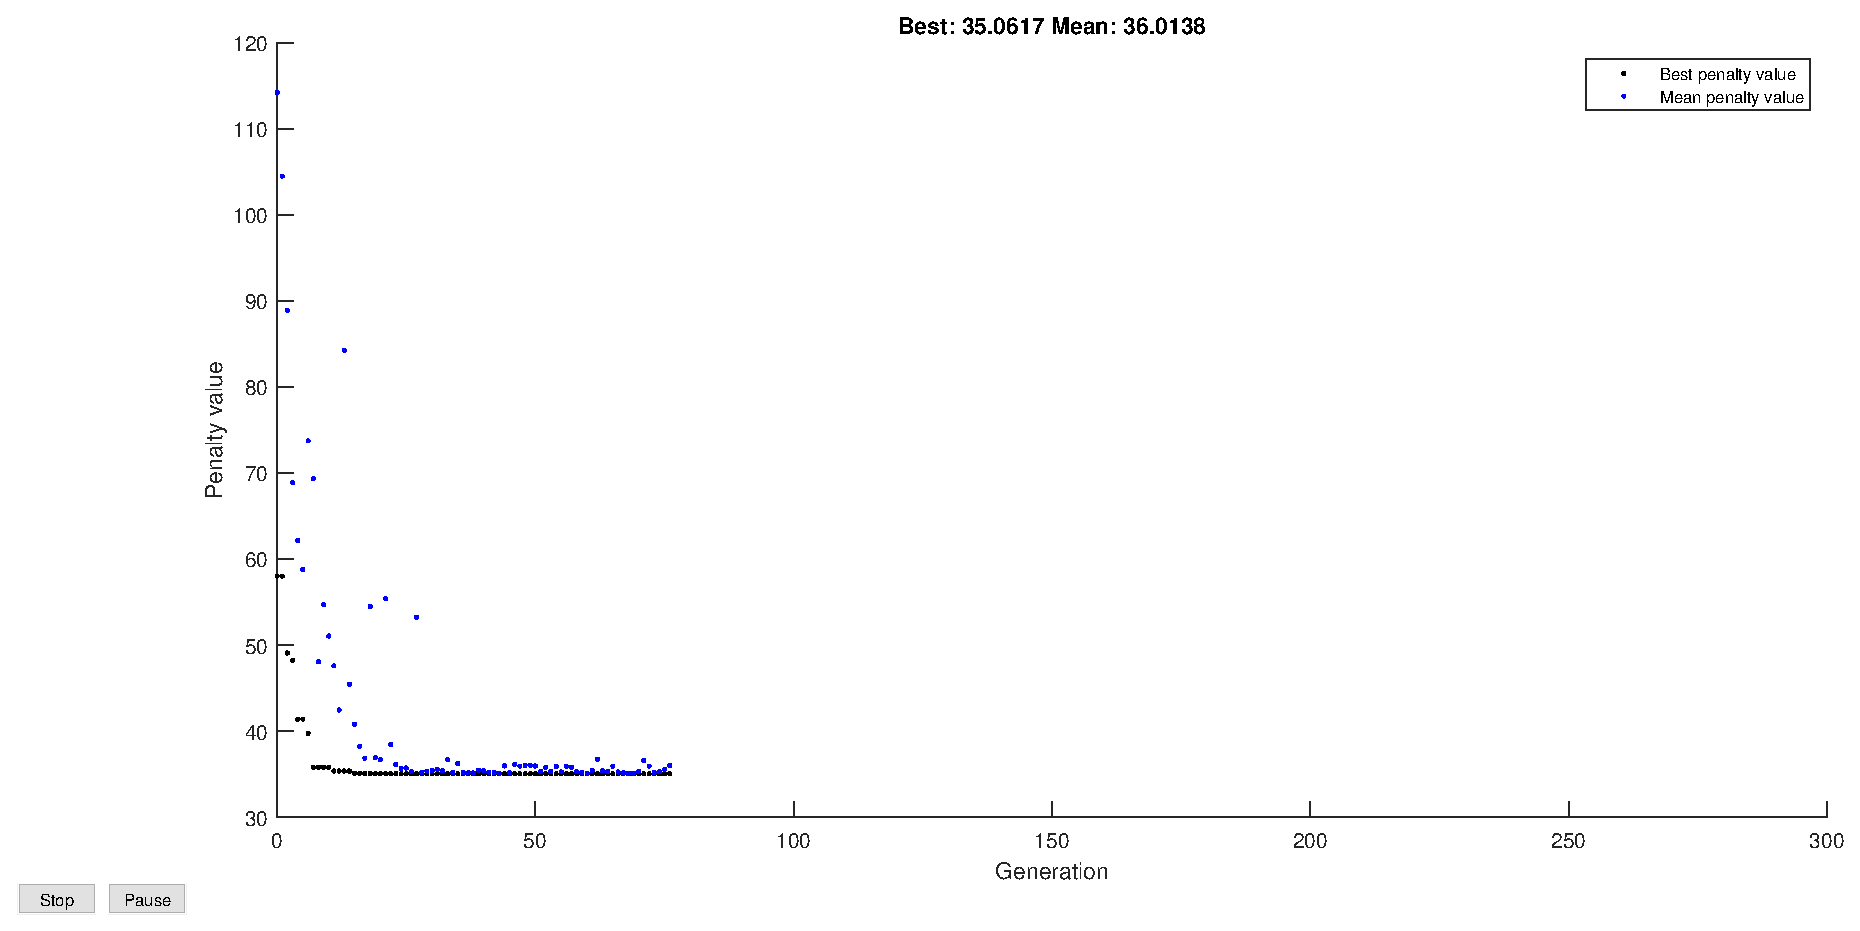
\includegraphics[scale=0.5]{Rys/strojenie.eps}
	\caption{Wyniki strojenia regulatora przy użyciu funkcji $ga$}
	\label{fig:strojenie}
\end{figure}

Przykładowy przebieg pokazujący pracę wystrojonego już regulatora można zobaczyć na wykresie \ref{fig:przebieg1}

\begin{figure}
	\centering
	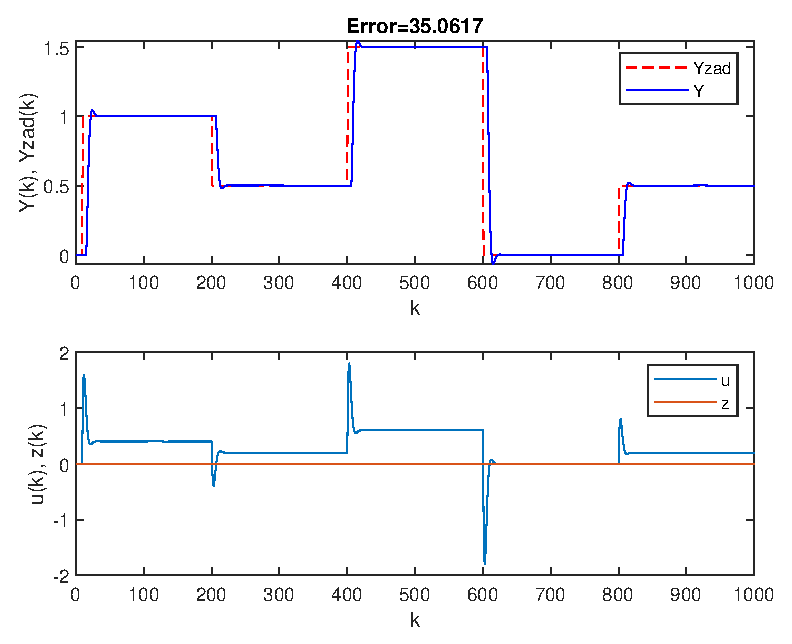
\includegraphics[scale=1]{Rys/przebieg1.eps}
	\caption{Przebieg dla parametrów $N = 116$, $N_u = 4$, $\lambda = 1$}
	\label{fig:przebieg1}
\end{figure}
